%%%%%%%%%%%%%%%%%%%%%%%%%%%%%%%%%%%%%%%%%
% University/School Laboratory Report
% LaTeX Template
% Version 4.0 (March 21, 2022)
%
% This template originates from:
% https://www.LaTeXTemplates.com
%
% Authors:
% Vel (vel@latextemplates.com)
% Linux and Unix Users Group at Virginia Tech Wiki
%
% License:
% CC BY-NC-SA 4.0 (https://creativecommons.org/licenses/by-nc-sa/4.0/)
%
%%%%%%%%%%%%%%%%%%%%%%%%%%%%%%%%%%%%%%%%%

%----------------------------------------------------------------------------------------
%	PACKAGES AND DOCUMENT CONFIGURATIONS
%----------------------------------------------------------------------------------------

\documentclass[
	letterpaper, % Paper size, specify a4paper (A4) or letterpaper (US letter)
	10pt, % Default font size, specify 10pt, 11pt or 12pt
]{CSUniSchoolLabReport}

%----------------------------------------------------------------------------------------
%	REPORT INFORMATION
%----------------------------------------------------------------------------------------

\title{ECE 398-MA \\ Introduction to Modern Communication with Python and SDR \\ Lab 7 -- Frame Synchronization and DBPSK} % Report title

\author{Noah Breit} % Author name(s), add additional authors like: '\& James \textsc{Smith}'

\date{\today} % Date of the report

%----------------------------------------------------------------------------------------

\begin{document}

\maketitle % Insert the title, author and date using the information specified above

% \begin{center}
% 	\begin{tabular}{l r}
% 		Date Performed: & February 13, 2022 \\ % Date the experiment was performed
% 		Partners: & Cecilia \textsc{Smith} \\ % Partner names
% 		& Tajel \textsc{Khumalo} \\
% 		Instructor: & Professor \textsc{Rivera} % Instructor/supervisor
% 	\end{tabular}
% \end{center}

% If you need to include an abstract, uncomment the lines below
%\begin{abstract}
%	Abstract text
%\end{abstract}

%----------------------------------------------------------------------------------------
%	OBJECTIVE
%----------------------------------------------------------------------------------------

\section{Assignment 1}

\begin{lstlisting}[language=Python]
	import numpy as np
	import matplotlib.pyplot as plt
	from scipy.signal import butter, filtfilt, find_peaks, resample_poly
	
	def rrcosfilter(N, alpha, Tb, Fs):
	"""
	Generates a root raised cosine (RRC) filter (FIR) impulse response.
	
	Parameters
	----------
	N : int
	Length of the filter in samples.
	
	alpha : float
	Roll off factor (Valid values are [0, 1]).
	
	Tb : float
	Symbol period.
	
	Fs : float
	Sampling Rate.
	
	Returns
	---------
	h_rrc : 1-D ndarray of floats
	Impulse response of the root raised cosine filter.
	"""
	
	T_delta = 1/float(Fs)
	sample_num = np.arange(N)
	h_rrc = np.zeros(N, dtype=float)
	
	for x in sample_num:
	t = (x-N/2)*T_delta
	if t == 0.0:
	h_rrc[x] = 1.0 - alpha + (4*alpha/np.pi)
	elif alpha != 0 and t == Tb/(4*alpha):
	h_rrc[x] = (alpha/np.sqrt(2))*(((1+2/np.pi)* (np.sin(np.pi/(4*alpha)))) + ((1-2/np.pi)*(np.cos(np.pi/(4*alpha)))))
	elif alpha != 0 and t == -Tb/(4*alpha):
	h_rrc[x] = (alpha/np.sqrt(2))*(((1+2/np.pi)* (np.sin(np.pi/(4*alpha)))) + ((1-2/np.pi)*(np.cos(np.pi/(4*alpha)))))
	else:
	h_rrc[x] = (np.sin(np.pi*t*(1-alpha)/Tb) +
	4*alpha*(t/Tb)*np.cos(np.pi*t*(1+alpha)/Tb))/ (np.pi*t*(1-(4*alpha*t/Tb)*(4*alpha*t/Tb))/Tb)
	
	return h_rrc
	
	
	# Create random binary data and BPSK symbols from the previous labs
	num_data_symbols = 32
	sps = 16
	
	np.random.seed(0)
	bits = np.random.randint(0, 2, num_data_symbols) # 0 to 1
	print(bits)
	print(np.sum(bits))
	bpsk_symbols = bits*2 - 1
	
	############ YOUR CODE STARTS HERE ############
	preamble = np.array([1,1,1,1,1,-1,-1,1,1,-1,1,-1,1])
	# Concatenate preamble, guard interval, and data symbols to create a frame here
	guard_interval = np.zeros(len(preamble))
	frame = np.concatenate([preamble, guard_interval, bpsk_symbols])
	# Upsample and perform pulse-shaping here (the pulse is given)
	
	# Tx_ADC is the pulse-shaped signal
	
	num_taps = 6*sps + 1
	pulse = rrcosfilter(N=num_taps, alpha=1.0, Tb=sps, Fs=1)
	frame_upsampled = np.zeros(len(frame) * sps)
	frame_upsampled[::sps] = frame
	Tx_ADC = np.convolve(frame_upsampled, pulse)
	
	############ YOUR CODE ENDS HERE ############
	
	
	############################################
	## Simulate IQ modulator (Tx)
	############################################
	
	M = 16  # upsample fs_adc for pass-band simulation
	xup = resample_poly(Tx_ADC, M, 1)
	
	
	fs_adc = sps    # sampling rate of ADC
	fs_rf = M * fs_adc  # sampling rate for simulating carrier
	fc = (M*3/7) * fs_adc # carrier frequency
	
	t = 1/fs_rf*np.arange(len(xup)) # time vector at fs_rf
	
	
	# u(t): transmitted signal to the channel (passband)
	u = np.real(xup) * np.cos(2*np.pi*fc*t) - np.imag(xup) * np.sin(2*np.pi*fc*t)
	
	############################################
	## Simulate Channel
	############################################
	ch_att = 0.1    # channel attenuation
	
	h = np.zeros(M*sps)
	h[0] = ch_att
	h = np.roll(h, np.random.randint(M*sps))    # random delay
	
	v = np.convolve(u, h) 
	noise_amplitude = 0.01
	noise = noise_amplitude * np.random.randn(len(v))   # AWGN
	
	v = v + noise
	
	
	
	############################################
	## Simulate IQ demodulator (Rx)
	############################################
	# Low-Pass Filter (LPF) @ fc
	Nfilt = 5
	cutoff = fc
	b, a = butter(Nfilt, Wn=cutoff, btype='low', fs=fs_rf)
	
	t = 1/fs_rf*np.arange(len(v))
	
	yI = filtfilt(b, a, v*np.cos(2*np.pi*fc*t))
	yQ = filtfilt(b, a, v*np.sin(2*np.pi*fc*t))
	
	Rx_ADC = resample_poly(yI + 1j*yQ, 1, M)
	############ YOUR CODE ENDS HERE ############
	# Tx, Channel, and raw Rx samples from the previous part
	
	############ YOUR CODE STARTS HERE ############
	# Matched filtering and symbol timing recovery from the previous labs here
	matched_filter = pulse
	rx_matched = np.convolve(Rx_ADC, matched_filter)
	# Frame synchronization: compute cross-correlation and detect the peak  
	preamble_upsampled = np.zeros(len(preamble)*sps)
	preamble_upsampled[::sps] = preamble
	# correlation = np.abs(np.correlate(rx_matched, preamble_upsampled, mode='valid')) / len(preamble_upsampled)
	correlation = np.abs(np.convolve(rx_matched, preamble_upsampled[::-1])) / len(preamble_upsampled)
	# Plot the cross-correlation and its peak
	peak_idx = correlation.argmax()
	start_idx = peak_idx + len(preamble_upsampled)
	print("Assignment1b:")
	print("Peak Index: ", peak_idx)
	print("Frame Start Index: ", start_idx)
	plt.figure(figsize=(10, 5))
	plt.plot(correlation, label='Cross-Correlation')
	plt.plot(peak_idx, correlation[peak_idx], 'rx', label=f'Peak={peak_idx}')
	plt.plot(start_idx, correlation[start_idx], 'rX', label=f'FrameStart={start_idx}')
	plt.title('Cross-Correlation and Detected Peak and Frame Start')
	plt.xlabel('Sample Index')
	plt.ylabel('Correlation')
	plt.legend()
	plt.grid(True)
	plt.savefig('assignment1a.png')
	plt.show()
	# Plot the IQ constellation
	rx_data = rx_matched[start_idx:start_idx + num_data_symbols*sps]
	plt.figure
	plt.plot(rx_data.real, rx_data.imag, '.')
	plt.xlabel('I')
	plt.ylabel('Q')
	plt.title('Received Data Constellation')
	plt.grid(True)
	ax = plt.gca()
	ax.set_aspect('equal', adjustable='datalim')
	plt.savefig('assignment1b.png')
	plt.show()
	############ YOUR CODE ENDS HERE ############
\end{lstlisting}

\begin{figure}[H] % [H] forces the figure to be placed exactly where it appears in the text
	\centering % Horizontally center the figure
	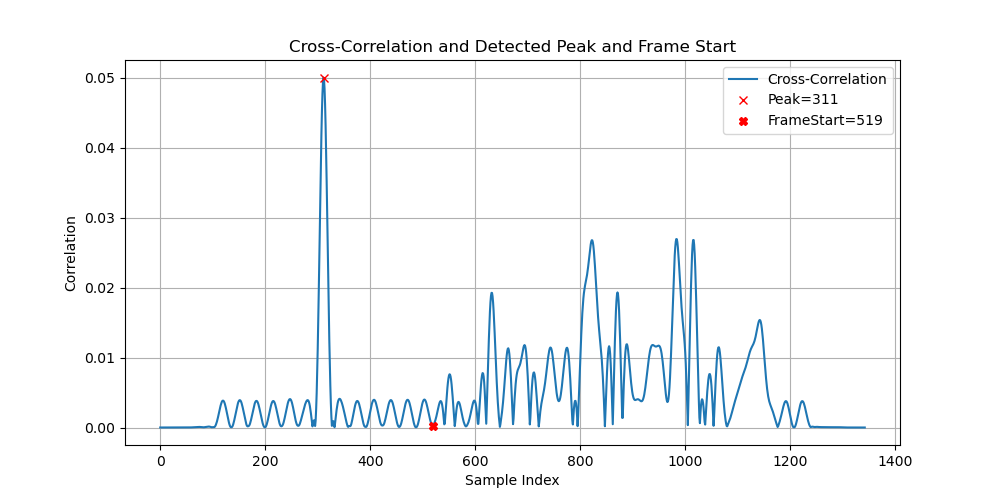
\includegraphics[width=1.2\textwidth]{assignment1a.png} % Include the figure
	\caption{Cross-Correlation of received Preamble+BPSK Symbols}
	\label{fig:block}
\end{figure}

Assignment1b:\newline
Peak Index:  311\newline
Frame Start Index:  519

\begin{figure}[H] % [H] forces the figure to be placed exactly where it appears in the text
	\centering % Horizontally center the figure
	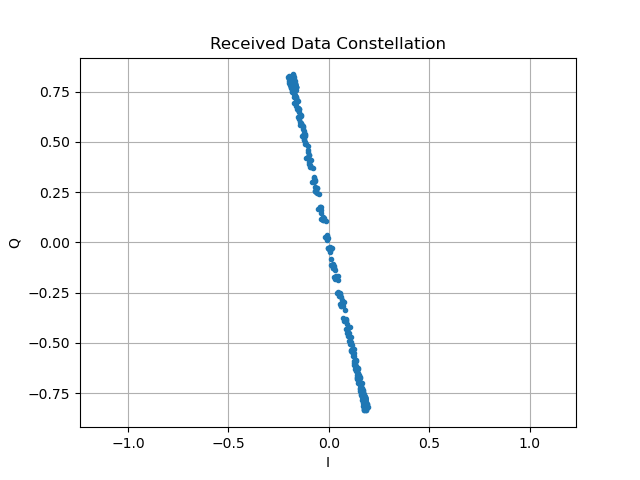
\includegraphics[width=1.2\textwidth]{assignment1b.png} % Include the figure
	\caption{BPSK Constellation}
	\label{fig:block}
\end{figure}

\section{Assignment 2}

\begin{lstlisting}[language=Python]
	
	################### PART 2 #####################
	
	# 1. DBPSK Transmitter
	# Convert BPSK symbols to DBPSK symbols
	dbpsk_symbols = np.zeros(len(bits) + 1)
	dbpsk_symbols[0] = 1  # Initialize the reference DBPSK symbol
	for k in range(len(bits)):
	dbpsk_symbols[k+1] = dbpsk_symbols[k] * bpsk_symbols[k]  # Differential encoding
	
	# Create frame with preamble and guard interval (same as BPSK)
	frame_dbpsk = np.concatenate([preamble, guard_interval, dbpsk_symbols])  # Skip reference symbol
	
	# Upsample and apply pulse shaping
	frame_upsampled_dbpsk = np.zeros(len(frame_dbpsk) * sps)
	frame_upsampled_dbpsk[::sps] = frame_dbpsk
	Tx_ADC_dbpsk = np.convolve(frame_upsampled_dbpsk, pulse)
	
	# 2. Transmit through channel (reuse channel code from Part 1)
	############################################
	## Simulate IQ modulator (Tx)
	############################################
	
	M = 16  # upsample fs_adc for pass-band simulation
	xup = resample_poly(Tx_ADC_dbpsk, M, 1)
	
	
	fs_adc = sps    # sampling rate of ADC
	fs_rf = M * fs_adc  # sampling rate for simulating carrier
	fc = (M*3/7) * fs_adc # carrier frequency
	
	t = 1/fs_rf*np.arange(len(xup)) # time vector at fs_rf
	
	
	# u(t): transmitted signal to the channel (passband)
	u = np.real(xup) * np.cos(2*np.pi*fc*t) - np.imag(xup) * np.sin(2*np.pi*fc*t)
	
	############################################
	## Simulate Channel
	############################################
	ch_att = 0.1    # channel attenuation
	
	h = np.zeros(M*sps)
	h[0] = ch_att
	h = np.roll(h, np.random.randint(M*sps))    # random delay
	
	v = np.convolve(u, h) 
	noise_amplitude = 0.01
	noise = noise_amplitude * np.random.randn(len(v))   # AWGN
	
	v = v + noise
	
	############################################
	## Simulate IQ demodulator (Rx)
	############################################
	# Low-Pass Filter (LPF) @ fc
	Nfilt = 5
	cutoff = fc
	b, a = butter(Nfilt, Wn=cutoff, btype='low', fs=fs_rf)
	
	t = 1/fs_rf*np.arange(len(v))
	
	yI = filtfilt(b, a, v*np.cos(2*np.pi*fc*t))
	yQ = filtfilt(b, a, v*np.sin(2*np.pi*fc*t))
	
	Rx_ADC_dbpsk = resample_poly(yI + 1j*yQ, 1, M)
	
	# 3. DBPSK Receiver
	# Apply matched filtering (same as BPSK)
	rx_matched_dbpsk = np.convolve(Rx_ADC_dbpsk, matched_filter)
	
	# Frame synchronization (same as BPSK)
	correlation_dbpsk = np.abs(np.convolve(rx_matched_dbpsk, preamble_upsampled[::-1])) / len(preamble_upsampled)
	peak_idx_dbpsk = correlation_dbpsk.argmax()
	start_idx_dbpsk = peak_idx_dbpsk + len(preamble_upsampled)
	
	# DEBUGGING
	plt.figure(figsize=(10, 5))
	plt.plot(correlation_dbpsk, label='Cross-Correlation')
	plt.plot(peak_idx_dbpsk, correlation_dbpsk[peak_idx_dbpsk], 'rx', label=f'Peak={peak_idx_dbpsk}')
	plt.plot(start_idx_dbpsk, correlation_dbpsk[start_idx_dbpsk], 'rX', label=f'FrameStart={start_idx_dbpsk}')
	plt.title('Cross-Correlation and Detected Peak and Frame Start')
	plt.xlabel('Sample Index')
	plt.ylabel('Correlation')
	plt.legend()
	plt.grid(True)
	plt.show()
	
	# Extract and downsample symbols
	rx_symbols_dbpsk = rx_matched_dbpsk[start_idx_dbpsk:start_idx_dbpsk + num_data_symbols*sps + 1:sps]
	
	# DBPSK demodulation - calculate phase difference
	demod_symbols = np.zeros(len(bits), dtype=complex)
	for k in range(1, len(rx_symbols_dbpsk)):
	demod_symbols[k-1] = rx_symbols_dbpsk[k] * np.conj(rx_symbols_dbpsk[k-1])  # Phase difference
	
	# Convert to bits
	received_bits_dbpsk = (np.real(demod_symbols) < 0).astype(int)
	
	# 4. Results and Comparison
	# Calculate Bit Error
	ber_dbpsk = np.sum(bits != received_bits_dbpsk) / len(bits)
	
	# Print results
	print("Assignment2b:")
	print("Original bits:  ", bits)
	print("DBPSK received: ", received_bits_dbpsk)
	print("Assignment2c:")
	print(f"DBPSK BER: {ber_dbpsk:.4f}")
	
	# Plot constellations
	plt.figure(figsize=(10, 5))
	plt.subplot(121)
	plt.plot(rx_data.real, rx_data.imag, '.')
	plt.title('BPSK Constellation')
	plt.grid(True)
	plt.axis('equal')
	
	plt.subplot(122)
	plt.plot(rx_symbols_dbpsk.real, rx_symbols_dbpsk.imag, '.')
	plt.title('DBPSK Constellation')
	plt.grid(True)
	plt.axis('equal')
	plt.tight_layout()
	plt.savefig('assignment2a.png')
	plt.show()
\end{lstlisting}

\begin{figure}[H] % [H] forces the figure to be placed exactly where it appears in the text
	\centering % Horizontally center the figure
	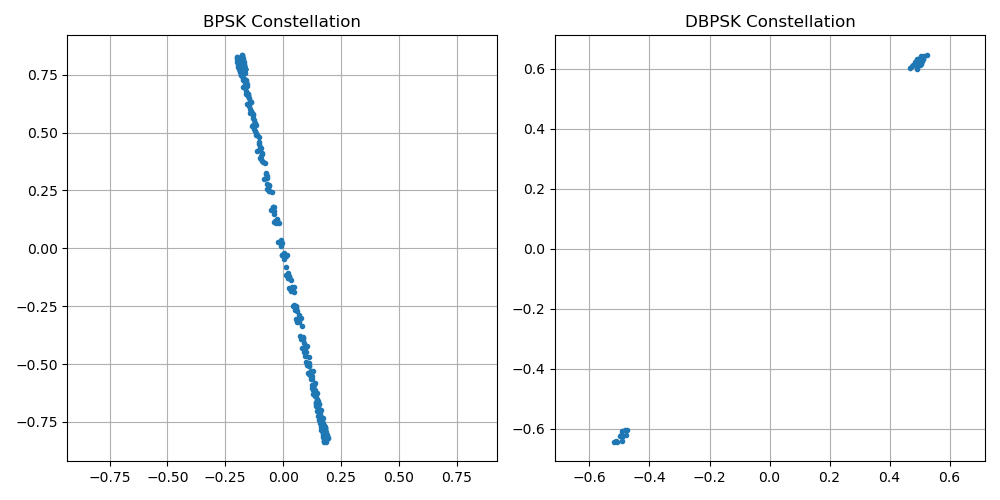
\includegraphics[width=1.2\textwidth]{assignment2a.png} % Include the figure
	\caption{BPSK and DBPSK Constellations}
	\label{fig:block}
\end{figure}

Assignment2b: \newline
Original bits:   [0 1 1 0 1 1 1 1 1 1 1 0 0 1 0 0 0 0 0 1 0 1 1 0 0 1 1 1 1 0 1 0]\newline
DBPSK received:  [0 1 1 0 1 1 1 1 1 1 1 0 0 1 0 0 0 0 0 1 0 1 1 0 0 1 1 1 1 0 1 0]\newline

Assignment2c: \newline
DBPSK BER: 0.0000

\end{document}